\subsection{Maximum Speed}
When an object is in a vacant time interval its position can be narrowed further down then the cell it is presumer to be located in. 
This is done based on the max speed of the object which is $V_{max}*\Delta t_1$ . 
We view the range of the sensor $s$ as a circle with the sensors maximum range as radious, we call this $r_1$. 
Knowing the maximum speed of the object a circle can be drawn from the point where the object lef the vacinity of the sensor.
This circle is the area where the object is located. 
It is, however, not know the point of exit from the sensor but only that the object left. 
The area of the object can then be calculated by creating a circle with the maximum sensor range plus the maximum range that the object can have traveled. 





\begin{figure}%
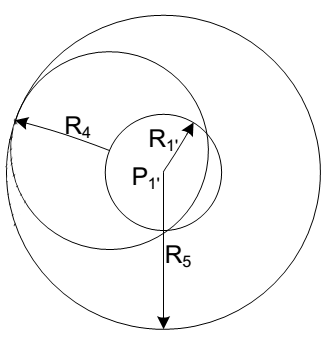
\includegraphics{images/speed.png}%
\caption{}%
\label{}%
\end{figure}
